\documentclass[conference]{IEEEtran}
\IEEEoverridecommandlockouts

\usepackage{amssymb}
\usepackage[table]{xcolor}
\usepackage{xspace}
\usepackage{booktabs}
\usepackage{amsmath}
\usepackage{graphicx}
\usepackage{algorithm}
\usepackage{algpseudocode}
\usepackage{float}
\usepackage{cite}
\usepackage{subcaption}
\usepackage{makecell}
\usepackage{array}    % better column types (p{}, >{...})
\usepackage{tabularx} % tables that fit \columnwidth
\usepackage{xurl}
\usepackage{tikz}
\usetikzlibrary{arrows.meta, positioning, fit, calc}
% ---- Macros ----
\newcommand{\smarm}{SMARM\xspace}
\newcommand{\tdis}{$t_{\mathrm{disabled}}$\xspace}
\newcommand{\FAR}{FAR\xspace}
\newcommand{\smarmcopy}{SMARM-Snap\xspace}
\newcommand{\smarmlock}{SMARM-Guard\xspace}

\newcommand\oak[1]{\textcolor{red}{OAK: #1}}
% \newcommand\oak[1]{}
\newcommand\todo[1]{\textcolor{red}{TODO: #1}}
\newcommand\ignore[1]{}
\newcommand\ben[1]{\textcolor{blue}{#1}}
% \newcommand\ben[1]{#1}


% \setlength{\columnsep}{0.24in} % gutter between columns

%Ben
\setlength{\textfloatsep}{6pt plus 2pt minus 2pt}
\setlength{\floatsep}{6pt plus 2pt minus 2pt}
\setlength{\intextsep}{6pt plus 2pt minus 2pt}
\setlength{\abovecaptionskip}{3pt}
\setlength{\belowcaptionskip}{0pt}

% \setlength{\textfloatsep}{4pt plus 1pt minus 2pt}
% \setlength{\floatsep}{4pt plus 1pt minus 2pt}
% \setlength{\intextsep}{4pt plus 1pt minus 2pt}
% \setlength{\abovecaptionskip}{2pt}
% \setlength{\belowcaptionskip}{0pt}



% Pull references up a bit (avoid an extra mostly-empty last page)
% \setlength{\textfloatsep}{9pt plus 2pt minus 2pt}
% \setlength{\floatsep}{8pt plus 2pt minus 2pt}
% \setlength{\intextsep}{8pt plus 2pt minus 2pt}
% \setlength{\abovecaptionskip}{6pt}
% \setlength{\belowcaptionskip}{1pt}

\usepackage[top=0.75in, bottom=1.1in, left=0.625in, right=0.625in]{geometry}
\begin{document}

\title{Towards Fully Interruptible Shuffled Measurement for Remote Attestation}

% DOUBLE-BLIND: comment out \author before submitting if required
\author{
  \IEEEauthorblockN{Amarin Laohajirapan, Norrathep Rattanavipanon}
  \IEEEauthorblockA{College of Computing,
    Prince of Songkla University, Phuket Campus, Thailand \\ 6730621007@psu.ac.th,
    norrathep.r@psu.ac.th}
}

\maketitle

% ================================================================
\begin{abstract}
Remote attestation (RA) detects software compromise on IoT devices, but
traditional RA keeps interrupts disabled for a full memory (hash) measurement and can block real-time workload for hundreds of milliseconds.
Prior work, called SMARM, instead measures memory in a private random order, so attestation can be interrupted between blocks while still resisting \emph{roving malware}.
As a result, SMARM reduces the non-interruptibility period from a full memory measurement to a single-block measurement.
Despite this improvement, this period can be non-negligible for large block sizes, making SMARM less ideal for deadline-driven or time-sensitive settings.
In this work, we propose two independent enhancements to SMARM that reduce this non-interruptibility period even further.
The first, called \emph{\smarmcopy}, disables interrupts only around a short memory copy into Secure RAM, then hashes the copied block with interrupts enabled.
The second, \emph{\smarmlock}, instead makes the target block temporarily inaccessible to Non-Secure software during an in-place hash, with no copy buffer.
% On STM32L552ZE with FreeRTOS, both substantially reduce the per-block
% interrupt-disabled window for block sizes up to $B{=}4096$~bytes;
% using the Frequency Accuracy Ratio (FAR) from prior FreeRTOS/TrustZone-M
% SMARM work, we also observe FAR~$\approx 1.0$ under a $1000$~Hz workload.
% OLD:
% On STM32L552ZE with FreeRTOS, both substantially reduce the non-interruptibility period even for large block sizes, i.e., by one order of magnitude with \smarmcopy{} and by two to three in \smarmlock.
On STM32L552ZE with FreeRTOS, both substantially reduce the non-interruptibility period even for large block sizes: by about one order of magnitude ($\sim\!\!15\times$) with \smarmcopy{} and by roughly three to four orders of magnitude with \smarmlock{} at 4KiB block size. 
%Measured FAR under a $1000$~Hz FreeRTOS task remains $1.0$ for both enhancements across all tested~$B$.
\end{abstract}

\begin{IEEEkeywords}
Remote attestation, shuffled measurement, IoT security, TrustZone-M
\end{IEEEkeywords}

% ================================================================
\section{Introduction}
\label{sec:intro}

Modern societies increasingly depend on Internet-of-Things (IoT) devices across domains ranging from smart factories, where industrial sensors support monitoring and automation, to smart homes, where devices such as smart lights and robotic vacuum cleaners improve convenience. 
Since many IoT devices are designed to be inexpensive and energy-efficient, they typically operate on resource-constrained microcontrollers (MCUs) with limited RAM, flash storage, and energy budgets. These constraints often preclude sophisticated monolithic operating systems and the malware defenses available on higher-end devices (e.g., desktop computers or servers).

Remote attestation (RA)~\cite{eldefrawy2012smart,nunes2019vrased,eldefrawy2017hydra} has emerged as an inexpensive technique for detecting malware compromise on resource-constrained IoT devices. In RA, an IoT device, called the \emph{prover}, executes a measurement routine that hashes its software image (i.e., the code stored in flash memory) and returns the measurement result in an authenticated response, e.g., using a message authentication code (MAC). 
An external trusted party, called the \emph{verifier}, authenticates this response and then compares the measurement against that of the expected software image to determine whether the prover's software has been modified and hence whether a malware compromise has occurred on the prover.

Traditional RA requires the measurement routine to execute atomically with interrupts disabled~\cite{eldefrawy2012smart,nunes2019vrased,francillon2014minimalist}. This atomic execution is necessary to prevent \emph{roving malware} from evading detection by relocating itself to a region that has already been measured. On low-end MCUs, however, the resulting non-interruptibility period can exceed $450$~ms~\cite{nunes2019vrased}. Such prolonged interrupt disablement can severely interfere with real-time applications whose correctness depends on completing time-critical tasks within their deadlines.

To relax the atomicity requirement, SMARM~\cite{carpent2018smarm} introduces a new technique, called \emph{shuffled measurement}, which permits interrupts between the measurements of individual memory blocks. To defend against roving malware, SMARM measures the blocks comprising the software image in a random and secret order. Since malware does not know which blocks have already been measured, it cannot reliably relocate itself to an inspected block to evade detection. Although this approach does not provide the deterministic protection of fully atomic measurement, it makes evasion probabilistically difficult while reducing the non-interruptibility period from the measurement of the entire software image to that of a single block.

Despite this improvement, SMARM's maximum non-interruptibility period remains determined by its block size. Prior work~\cite{smarmplus2026,carpent2018smarm} shows that using larger blocks can reduce the total attestation time by lowering per-block processing overhead. However, a larger block also takes longer to measure, thereby extending each non-interruptibility period and potentially delaying time-critical tasks beyond their deadlines. Conversely, smaller blocks shorten these intervals but increase the number of blocks and the associated computational overhead, resulting in longer attestation times and higher energy consumption. SMARM therefore exposes an inherent tradeoff between real-time responsiveness and energy efficiency, which is particularly problematic for energy-constrained (e.g., battery-powered) IoT devices.


Motivated by this observation, we propose two independent enhancements to shuffled measurement that further shorten its non-interruptibility periods, allowing the technique to coexist with a broader range of time-sensitive applications.
Our contributions are as follows:

\begin{itemize}
\item We propose \smarmcopy, which reduces each non-interruptibility period from the time required to hash one memory block to the substantially shorter time required to take a snapshot of (i.e., perform a memory copy of) that block.

 

\item \smarmcopy incurs additional Secure RAM to hold a copied block. To relax this constraint, we propose \smarmlock, which disables interrupts only for temporarily changing the security attribute of the memory block without copying its contents.
As an additional benefit, \smarmlock further reduces the non-interruptibility period,
at the cost of potentially interfering with concurrent Non-Secure memory accesses
to the guarded block.

% \item We implement \smarmcopy and \smarmlock on an STM32 Nucleo-144 board (STM32L552ZE, Cortex-M33 with TrustZone-M)~\cite{stm32nucleo144} running FreeRTOS and evaluate them on real hardware. Our results demonstrate that both mechanisms substantially reduce SMARM's non-interruptibility periods by 1-3 orders of magnitude, thereby improving its compatibility with time-sensitive embedded applications.
\item We implement and evaluate \smarmcopy and \smarmlock on an STM32 Nucleo-144 board~\cite{stm32nucleo144} running FreeRTOS. Our results show that \smarmcopy{} reduces the non-interruptibility
period by about one order of magnitude and \smarmlock{} by roughly
three to four orders for large block sizes.


\end{itemize}


\section{Background}
\label{sec:background}

\subsection{RA Atomicity and SMARM}

%\oak{Briefly mention RA workflow, i.e., challenge-response between prover and verifier etc.}
At a high level, remote attestation (RA) is a challenge--response
protocol between a \emph{prover} (i.e., a resource-constrained IoT device in this work) and a trusted \emph{verifier}.
The verifier sends a fresh challenge (e.g., a random nonce); 
the prover computes an authenticated integrity measurement, typically using a message authentication code (MAC), over its software image together with that challenge and a pre-shared attestation key $k$ and returns it as attestation evidence. 
The verifier then checks the evidence using the verification key against a reference value for the expected software state.
Classical RA techniques often \emph{disable interrupts} for the whole measurement so that \emph{roving malware} cannot move itself while memory is being hashed~\cite{eldefrawy2012smart,nunes2019vrased}.
This makes those techniques undesirable for time-sensitive or deadline-driven settings.

To address this, SMARM~\cite{carpent2018smarm} partitions the attested
memory region $M$ into fixed-size blocks of $B$ bytes and derives a
one-time permutation $\sigma$ from $k$ and the verifier challenge.
It then measures the blocks $M_{\sigma[i]}$ one by one, re-enabling
interrupts between consecutive block measurements.
The security claim is not ``malware cannot interrupt''; it is that without knowledge of the remaining secret order, malware cannot reliably relocate to escape detection, and repeated independent sessions drive the escape probability down.
SMARM requires the following security properties:
\begin{enumerate}
  % \item[\textbf{[S1]}] \textbf{Controlled Execution.}
  %   The attestation function (i.e., the authenticated integrity and measurement routines) is reachable only through defined
  %   entry/exit points. Interrupts may be re-enabled only
  %   \emph{between} block measurements so malware cannot relocate itself during a block measurement.
    \item[\textbf{[S1]}] \textbf{Controlled Execution.}
    The attestation function is reachable only through defined entry and
    exit points. Interrupts may be re-enabled only
    between complete block measurements so that untrusted software cannot interfere with an ongoing block measurement.
    
  \item[\textbf{[S2]}] \textbf{Key Secrecy.}
    $k$ is stored in memory inaccessible to
    untrusted software, so malware cannot obtain it to directly forge a valid report without triggering the attestation function.
  \item[\textbf{[S3]}] \textbf{Private Measurement Order.}
    $\sigma$ is stored in memory inaccessible to malware such that the malware cannot predict which remaining blocks will be measured next and relocate before/after each block measurement.
\end{enumerate}
The original SMARM design builds on the HYDRA attestation architecture~\cite{eldefrawy2017hydra} to satisfy these properties.


\subsection{ARM TrustZone-M}

% ARM TrustZone-M for Cortex-M~\cite{trustzone2025,an5347} provides a trusted execution environment (TEE) for resource-constrained MCUs by partitioning the system into two isolated \emph{worlds}: the \emph{Secure} world, which hosts trusted code and device secrets, and the \emph{Non-Secure} world, which runs untrusted software, including the real-time operating system (RTOS) and applications.
% %
% 

ARM TrustZone-M for Cortex-M~\cite{trustzone2025} partitions the MCU into a \emph{Secure} world (trusted code and secrets) and a
\emph{Non-Secure} world (RTOS and applications).
This isolation is enforced in hardware through memory security attribution. 
In particular, TrustZone-M uses the \emph{Implementation Defined Attribution Unit} (IDAU) and the \emph{Security Attribution Unit} (SAU) to determine whether each address range is Secure, Non-Secure, or Non-Secure Callable (NSC). The IDAU is defined by the MCU implementation and is fixed by the device design, whereas the SAU is programmable by Secure software, allowing device vendors to configure the Secure/Non-Secure memory partition according to their application requirements.

An important property of the SAU is that memory not explicitly attributed as Non-Secure by either the SAU or IDAU is treated as \emph{Secure by default}. Consequently, memory intended to be accessible from the Non-Secure world must be explicitly covered by a corresponding Non-Secure attribution region. These SAU regions are typically configured by Secure firmware during system initialization. The number of programmable SAU regions is implementation-dependent and varies across Cortex-M devices (e.g., 8 regions in our target devices).
%
Once the memory attribution is configured, the MCU prevents Non-Secure software from directly accessing Secure memory. 
Non-Secure software may invoke only designated Secure entry points located in NSC regions. Invoking such an entry point causes the MCU to transition from the Non-Secure state to the Secure state, where the corresponding Secure service can execute.

Recent work~\cite{smarmplus2026} adapts SMARM to coexist with an RTOS (e.g., FreeRTOS~\cite{freertos2025}) while leveraging TrustZone-M to preserve SMARM's security guarantees. In this design, FreeRTOS and application tasks execute in the Non-Secure world, while the SMARM service, attestation key~$k$, and secret permutation~$\sigma$ reside in the Secure world. 
A Non-Secure wrapper (as a real-time task) may invoke the SMARM service through an NSC entry point, as illustrated in Fig.~\ref{fig:system_model}. During attestation, interrupts are enabled only between consecutive block measurements, allowing the RTOS to schedule other tasks, including high-priority real-time workloads. We adopt the TrustZone-M-based SMARM design proposed in~\cite{smarmplus2026} as the baseline for this work.

\begin{figure}[htbp]
  \centering
  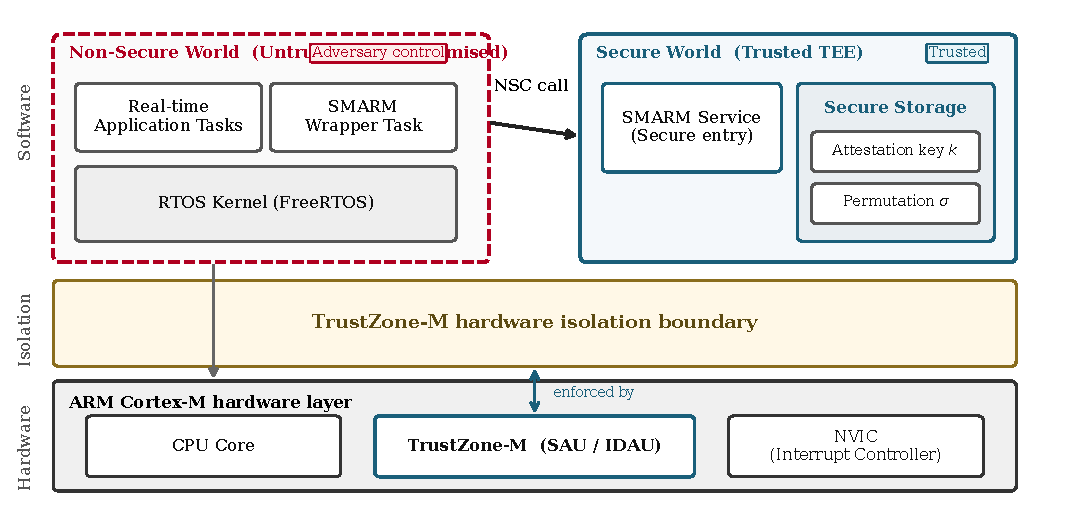
\includegraphics[width=1.0\linewidth]{system-threat-model.pdf}
  \caption{SMARM on FreeRTOS with TrustZone-M, as proposed in~\cite{smarmplus2026}.}
  \label{fig:system_model}
\end{figure}


% ================================================================
\section{Design}
\label{sec:design}

\subsection{Motivation}
\label{sec:motivation}

In the SMARM baseline, interrupts must be disabled throughout the measurement of each memory block. Consequently, the non-interruptibility period (\tdis), during which real-time tasks cannot execute, is determined by the time required to measure a single block. This duration depends primarily on two factors: the block size ($B$) and the measurement function.
%
% Following prior work~\cite{smarmplus2026,carpent2018smarm}, we investigated this issue using SHA-256 as the underlying measurement function. On an STM32 Nucleo-144 board, we observe that \tdis increases with $B$, from $0.062$~ms at $B{=}64$~bytes to $3.75$~ms at $B{=}4096$~bytes. For comparison, a high-frequency real-time task running at $1000$~Hz has a period of only 1~ms. Thus, with $B{=}4096$~bytes, a single SMARM block measurement can
% span several task periods and cause the real-time task to miss multiple
% deadlines. This makes the SMARM baseline unsuitable for such
% time-sensitive workloads.
Following prior work~\cite{smarmplus2026,carpent2018smarm}, we use a software HMAC-SHA-256 implementation in the Secure world as the measurement function. On our Nucleo-144 board, baseline \tdis{} increases with $B$,
from $0.119$~ms at $B{=}128$~bytes to $3.73$~ms at $B{=}4096$~bytes
(Sec.~\ref{sec:eval}). For comparison, a $1000$~Hz real-time task has a period of only 1~ms. Thus, with $B{=}4096$~bytes, a single SMARM block measurement can span several task periods and cause the real-time task to miss multiple deadlines.

In this work, we observe that the atomic per-block measurement used by
SMARM baseline can be relaxed without sacrificing its security goal.
Our key observation is that what must be preserved during each block
measurement is the \emph{temporal consistency} of the measured contents:
the measurement must correspond to a consistent state of the block at
some point during the measurement~\cite{carpent2018temporal}.
The SMARM baseline achieves this by hashing the entire block atomically with
interrupts disabled.

\emph{However, disabling interrupts throughout the entire measurement is not the only way to fulfill this property.}
The key requirement is instead to ensure a consistent \emph{capture} of the block contents that serve as input to the hash. Based on this observation, we propose two alternative mechanisms, \smarmcopy and \smarmlock, that preserve such consistency while substantially shortening the non-interruptibility period and allowing the hash computation itself to remain interruptible. Figure~\ref{fig:timing_diagram} compares their non-interruptibility periods with those of traditional RA and the SMARM baseline.

\begin{figure}[htbp]
  \centering
  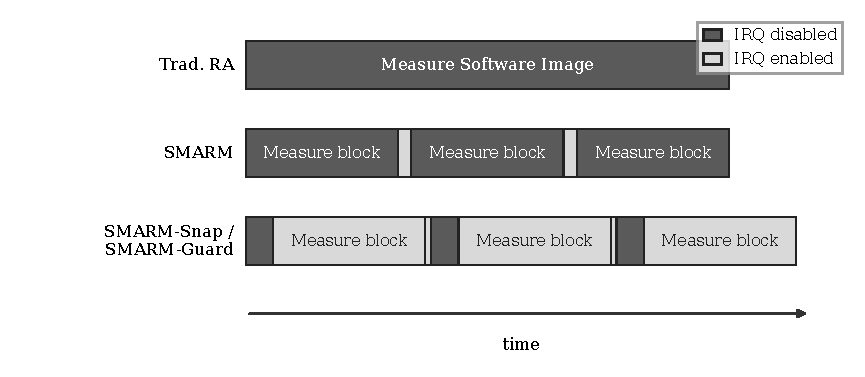
\includegraphics[width=1\linewidth]{timing_diagram.pdf}
  \caption{Comparison of non-interruptibility period between traditional RA, SMARM and our work.}
  \label{fig:timing_diagram}
 
\end{figure}

\subsection{System and Threat Model}
\label{sec:system_threat}

We follow the system and threat models of relevant prior work~\cite{smarmplus2026,rattanavipanon2025slapp}.
The prover is a resource-constrained IoT device equipped with a
TrustZone-M trusted execution environment (TEE).
It runs a commodity RTOS and application tasks in the Non-Secure world,
while a small Trusted Computing Base (TCB), including the attestation
service and its security-critical state, resides in the Secure world.
The remote verifier is trusted and aims to determine the integrity of
the prover's software while minimizing interference with real-time tasks
scheduled to run intermittently on the prover.

We consider a software-level adversary (i.e., malware) with full control
over the Non-Secure world, including the RTOS and applications.
In particular, the adversary may employ \emph{roving malware} that
relocates its malicious code during an ongoing attestation in an attempt
to evade measurement. The Secure world and its TCB are trusted; thus,
the adversary cannot compromise or modify code, data, or secrets residing
in Secure memory.
We consider hardware attacks, including attacks that directly manipulate
the hardware-enforced security attribution provided by the SAU/IDAU,
to be out of scope.

For \smarmlock{}, we assume that the attested region~$M$ is a dedicated
Non-Secure region that need not remain continuously accessible
to Non-Secure software during each block measurement.

\begin{figure*}[t]
  \centering
  \raisebox{-10pt}{
\includegraphics[width=\textwidth]{combined_workflow.pdf}}  \caption{Shared SMARM loop (left) with three per-block measurement
    options (right). Red dashed regions mark interrupt-disabled steps.
    SMARM baseline hashes under interrupts disabled; \smarmcopy{} copies
    under interrupts disabled then hashes with interrupts enabled;
    \smarmlock{} makes the selected block temporarily inaccessible to Non-Secure software via the SAU, hashes in place with interrupts enabled, then
    restores Non-Secure availability.}
  \label{fig:combined_workflow}
\end{figure*}




\subsection{\smarmcopy}
\label{sec:atomic}

Our first enhancement achieves temporal consistency by taking an atomic snapshot of the shuffled memory block to be measured ($M_{\sigma[i]}$) and storing the snapshot in Secure RAM, where it is inaccessible to untrusted Non-Secure software. The subsequent measurement is then performed over this Secure snapshot. We refer to this enhancement as \smarmcopy.

As illustrated in Fig.~\ref{fig:combined_workflow}, \smarmcopy follows the same overall workflow as the SMARM baseline and differs only in the per-block measurement operation. Rather than disabling interrupts for the entire measurement of $M_{\sigma[i]}$, \smarmcopy disables interrupts only while copying $M_{\sigma[i]}$ into Secure RAM.
Since the copy is performed atomically, the resulting snapshot corresponds to a consistent state of $M_{\sigma[i]}$.
Once the Secure snapshot is complete, interrupts can be re-enabled and the measurement function can operate on the snapshot without interference from untrusted software.

The direct benefit of \smarmcopy is that it substantially shortens \tdis, since \tdis is reduced from the time required to hash a block to the time required only to copy it. On our Cortex-M33 target, the memory-copy throughput is around $17$~MB/s, giving
$t_{\mathrm{disabled}}^{\mathrm{copy}}\approx B/(17~\mathrm{MB/s})$, which is about $15\times$ shorter than the corresponding \tdis of the SMARM baseline.
%
The main drawback of \smarmcopy{} is that it requires an additional
$B$ bytes of Secure RAM to hold the snapshot. Our second enhancement,
presented next, eliminates this additional Secure RAM overhead.



\subsection{\smarmlock}
\label{sec:sau}

While \smarmcopy achieves temporal consistency by copying each block into a Secure RAM buffer, this requires an additional $B$ bytes of Secure RAM. Our second enhancement, \smarmlock, avoids this storage overhead by making the memory block being measured, $M_{\sigma[i]}$, temporarily inaccessible to Non-Secure software.
This allows the SMARM service to measure the block \emph{in place} while interrupts remain enabled.

In our target system, we leverage the SAU to realize this mechanism. As shown in Figure~\ref{fig:combined_workflow}, before measuring $M_{\sigma[i]}$, \smarmlock reconfigures the SAU regions covering $M$ so that $M_{\sigma[i]}$ is excluded from Non-Secure coverage.
%The SAU configurations before and during block measurement are shown in Figure~\ref{fig:sau_memory_map}. 
Since memory not explicitly attributed as Non-Secure is considered to be Secure by default in TrustZone-M, this effectively makes $M_{\sigma[i]}$ accessible only from the Secure world. 
The SAU reconfiguration is followed by data and instruction synchronization barriers (\texttt{DSB} and \texttt{ISB}) to ensure that the new memory-security attribution takes effect immediately.

% To preserve temporal consistency, the SAU reconfiguration and the associated barriers must execute atomically with interrupts disabled. However, this atomic operation is substantially shorter than either hashing or copying the entire block.
% In our measurements, each SAU attribution update takes only
% $0.80$-$1.30\,\mu$s ($87$-$143$ cycles at $110$~MHz).
% Once the block has been guarded, interrupts are re-enabled and the SMARM service measures $M_{\sigma[i]}$ directly. During this period, Non-Secure software may continue executing but cannot access $M_{\sigma[i]}$.

% After the measurement completes, the SMARM service briefly disables interrupts to restore the original SAU configuration, making $M_{\sigma[i]}$ Non-Secure once again, and then proceeds to the next shuffled block $M_{\sigma[i+1]}$.
% Thus, \smarmlock reduces each non-interruptibility period to a short SAU reconfiguration operation while keeping the substantially longer measurement computation interruptible. Unlike \smarmcopy, it requires no additional Secure storage.
To preserve temporal consistency, each SAU reconfiguration and its
associated synchronization barriers must execute atomically with
interrupts disabled.

Before measuring $M_{\sigma[i]}$, \smarmlock{} disables interrupts,
reconfigures the SAU to make $M_{\sigma[i]}$ inaccessible to
Non-Secure software, and executes the required synchronization barriers.
Once this SAU reconfiguration is complete, interrupts are re-enabled
and the SMARM service measures $M_{\sigma[i]}$ directly. During this
period, Non-Secure software may continue executing but cannot access
$M_{\sigma[i]}$.

After the measurement completes, the SMARM service disables interrupts
again, restores the original SAU configuration, executes the
synchronization barriers, and re-enables interrupts before proceeding
to the next shuffled block $M_{\sigma[i+1]}$.

Thus, in \smarmlock{}, interrupts are disabled only during the SAU
reconfiguration and synchronization steps, while the in-place hash
executes with interrupts enabled. Unlike \smarmcopy{}, \smarmlock{}
requires no additional Secure RAM buffer.


\ignore{
\begin{figure}[!t]
  \centering
  \includegraphics[width=.8\linewidth]{sau_memory_map_compact.png}
  \caption{Non-Secure attribution of the attested flash before and
   during measurement. At rest, $|M|$ is fully Non-Secure; while
    $M_{\sigma(i)}$ is measured, two dynamic SAU regions leave the
    $B$-byte block uncovered (Secure by default). Interrupts are off
    only while the SAU is reprogrammed.}
  \label{fig:sau_memory_map}
\end{figure}
}


\ignore{
\begin{algorithm}[!ht]
\caption{\smarmlock{} Secure Service (TrustZone-M SAU instantiation)}
\label{alg:sau}
\begin{algorithmic}[1]
\Require $n$ blocks, shuffled indices $\sigma$, attested region $M$, key $k$
\State \Call{HMAC.Init}{$k$}
\State \Call{SAU.RestoreWindowNS}{$M$} \Comment{rest state: $|M|$ is NS}
\For{$i \gets 0$ to $n-1$}
  \State $\mathit{blk} \gets M[\sigma(i)\cdot B]$
  \State \Call{DisableInterrupts}{}
  \State \Call{SAU.LockBlock}{\textit{blk}, $B$} \Comment{R6/R7; blk Secure-by-default}
  \State \Call{DSB}{}; \Call{ISB}{}
  \State \Call{EnableInterrupts}{}
  \State \Call{HMAC.Update}{\textit{blk}, $B$} \Comment{in place; interrupts on}
  \State \Call{DisableInterrupts}{}
  \State \Call{SAU.RestoreWindowNS}{$M$}
  \State \Call{DSB}{}; \Call{ISB}{}
  \State \Call{EnableInterrupts}{}
\EndFor
\State \textbf{return} \Call{HMAC.Finalize}{}
\end{algorithmic}
\end{algorithm}
}



\subsection{Security Guarantees}
\label{sec:security_summary}

% Both \smarmcopy and \smarmlock modify only how each shuffled memory block is measured; they do not alter the underlying SMARM protocol. In particular, the attestation key $k$ and secret permutation $\sigma$ are generated, used, and stored exactly as in the SMARM baseline. Therefore, \textbf{[S2] Key Secrecy} and \textbf{[S3] Private Measurement Order} continue to hold. 
% Likewise, both designs preserve SMARM's controlled execution interface, where the attestation functionality remains within the Secure SMARM Service and can be invoked from the Non-Secure world only through its designated NSC entry point.


% The main change concerns \textbf{[S1] Controlled Execution}. In the SMARM baseline, interrupts are disabled throughout the measurement of each block, preventing malware from modifying or relocating the block while it is being hashed.
% Our designs shorten this non-interruptibility period while preserving the same requirement: \smarmcopy preserves \textbf{[S1]} because the atomic copy captures a consistent state of $M_{\sigma[i]}$ before any Non-Secure modification can occur, so subsequent changes to the original block cannot affect the already-copied snapshot. \smarmlock preserves \textbf{[S1]} without a copy by making $M_{\sigma[i]}$ inaccessible to Non-Secure software for the duration of the in-place hash such that malware cannot modify or relocate it during measurement.

% Thus, \smarmcopy and \smarmlock preserve \textbf{[S1]} through two different mechanisms.
% As such, with the unchanged guarantees of \textbf{[S2]} and \textbf{[S3]}, both enhancements retain the security guarantees of the SMARM baseline.



Both designs change only how temporal consistency is enforced for each shuffled block.
The SMARM service remains reachable from the Non-Secure world only via
the designated NSC entry, while key~$k$ and permutation~$\sigma$
remain protected in Secure memory.
With this, \textbf{[S1]} is preserved since \smarmcopy{} captures an atomic Secure snapshot before hashing with interrupts enabled, while \smarmlock{} makes $M_{\sigma[i]}$ inaccessible to Non-Secure software during the in-place hash.

% \textbf{[S2]} is still fulfilled since $k$ remains in Secure memory.
% The permutation~$\sigma$ also remains in Secure memory for both designs.
% \smarmcopy{} introduces no new observable signal about the current block, because hashing uses a Secure snapshot.
% For \smarmlock{}, however, concurrent Non-Secure accesses to a guarded block may exhibit distinguishable access or timing behavior and thereby reveal information about the current measurement block.
% We therefore do not claim baseline-equivalent order privacy for \smarmlock{} under active probing.
% Our evaluation uses a dedicated Non-Secure attested region (Section~\ref{sec:eval}); when continuous Non-Secure access is required during measurement, \smarmcopy{} or the SMARM baseline is preferable.
% Quantifying this leakage is left to future work.
\textbf{[S2]} is still fulfilled since $k$ remains in Secure memory.
%
For \textbf{[S3]}, the permutation~$\sigma$ remains in Secure memory
for both designs. \smarmcopy{} introduces no new observable signal
about the current block.
For \smarmlock{}, however, concurrent Non-Secure accesses to a guarded
block may exhibit distinguishable access or timing behavior and thereby
reveal information about the current measurement block. We therefore
do not claim baseline-equivalent order privacy for \smarmlock{} under
active probing.
Quantifying this leakage is left to future work.

% Our evaluation uses a dedicated Non-Secure attested region
% (Section~\ref{sec:eval}); when continuous Non-Secure access is required
% during measurement, \smarmcopy{} or the SMARM baseline is preferable.
% Quantifying this leakage is left to future work.
% \oak{please make sure you know what you are saying here... Don't just let AI copy-paste this to you.}



\section{Evaluation}
\label{sec:eval}

\subsection{Setup}

We evaluate the SMARM baseline, \smarmcopy{}, and \smarmlock{} on an STM32 Nucleo-144 board (STM32L552ZE, TrustZone-M) running at $110$~MHz with FreeRTOS in the Non-Secure world. The MCU has $512$~KiB of flash, with $256$~KiB assigned to Secure flash and the other $256$~KiB to Non-Secure flash. We use a fixed dedicated Non-Secure attested region
$M$ of size $|M|{=}128$~KiB. In each attestation round, every block
in $M$ is measured once according to the secret permutation~$\sigma$.
The measurement function is software HMAC-SHA-256 executed. We evaluate using various block sizes $B\in\{128,256,512,1024,2048,4096\}$~bytes and report the
non-interruptibility period, additional Secure RAM overhead,
real-time availability, and end-to-end attestation runtime.

\subsection{Non-interruptibility Period}

% Figure~\ref{fig:tdisabled} compares \tdis{} of the SMARM baseline, \smarmcopy, and \smarmlock{} on a logarithmic scale. Across all three designs, \tdis{} increases with the block size $B$, as larger blocks require more work during the corresponding uninterruptible operation.

% Compared with the baseline, \smarmcopy{} reduces \tdis{} by approximately one order of magnitude (about $15\times$) by replacing the per-block hash within the interrupt-disabled period with a substantially faster memory copy. At $B{=}4096$~bytes, \tdis{} decreases from $3.75$~ms in the baseline to about $0.24$~ms with \smarmcopy.


% \smarmlock{} further reduces \tdis{} by limiting interrupt disablement to the short SAU reconfiguration operations required to protect and restore each block. At $B{=}4096$~bytes, \tdis{} is around $0.8$-$1.3\,\mu$s, corresponding to a reduction of roughly three orders of magnitude compared with the baseline.

% Overall, these results show that \smarmcopy{} and \smarmlock{} substantially shorten SMARM's non-interruptibility period, reducing it from the millisecond range in the baseline to the sub-millisecond and microsecond ranges, respectively.

% ----- OLD t_disabled measurement / prose / table (pre mean+std revision) -----
% To precisely measure \tdis of each approach, we rely on the Cortex-M Data Watchpoint and Trace (DWT) cycle counter
% in the Secure world to record $\mathrm{CYCCNT}$ at the beginning and end of each \tdis delimited by \texttt{\_\_disable\_irq} and \texttt{\_\_enable\_irq}.
% For the SMARM baseline, each measured \tdis contains one HMAC-SHA-256 update of
% size~$B$; for \smarmcopy{}, it contains the \texttt{memcpy} of size~$B$;
% Since \smarmlock{} contains two periods: one for SAU reconfiguration and the other for SAU restoration, we consider \tdis in \smarmlock to be the maximum of these two periods.\oak{is this correct?}
% We report both mean and maximum over all measured \tdis-s in each attestation round across ten rounds.\oak{wheres the maximum results in the figure/table?}\oak{standard deviation?}
% Figure~\ref{fig:tdisabled} and Table~\ref{tab:tdisabled} summarize the results. Baseline and \smarmcopy{} \tdis{} grow roughly linearly with~$B$ since the runtime of their underlying operations (hash or copy) are linearly dependent on $B$.
% \smarmlock{} remains nearly independent of~$B$, staying in the sub-microsecond to $\sim\!\!1\,\mu$s range; the small observed variation across~$B$ reflects measurement-level variability rather than block-size-dependent hashing, which occurs with interrupts enabled.\oak{this is why we should report std.}
% \oak{we should expand more about benefit of using \smarmcopy and \smarmlock.}
% At $B{=}4096$, mean \tdis{} falls from $3.73$~ms (baseline) to $0.243$~ms (\smarmcopy{}, $\sim\!\!15\times$) and to $0.65\,\mu$s mean / $1.08\,\mu$s max (\smarmlock{}, roughly three to four orders of magnitude).
% \begin{table}[t]
%   \centering
% \caption{Mean \tdis{}: the SMARM baseline/\smarmcopy{} in ms;
% \smarmlock{} mean SAU-reconfiguration duration in $\mu$s.}
%   \label{tab:tdisabled}
%   \small
%   \setlength{\tabcolsep}{3.5pt}
%   \begin{tabularx}{\columnwidth}{@{}lXXXXXX@{}}
%     \toprule
%     \textbf{$B$} & 128 & 256 & 512 & 1024 & 2048 & 4096 \\
%     \midrule
%     Baseline (ms) & 0.119 & 0.235 & 0.469 & 0.935 & 1.867 & 3.731 \\
%     \smarmcopy{} (ms) & 0.008 & 0.015 & 0.031 & 0.061 & 0.122 & 0.243 \\
%     \smarmlock{} ($\mu$s) & 0.40 & 0.41 & 0.42 & 0.45 & 0.52 & 0.65 \\
%     \bottomrule
%   \end{tabularx}
% \end{table}
% ----- end OLD -----

\paragraph{Measurement method}
To precisely measure \tdis{} for each approach, we use the Cortex-M
Data Watchpoint and Trace (DWT) cycle counter in the Secure world.
We record $\mathrm{CYCCNT}$ at the beginning and end of each
interrupt-disabled period delimited by
\texttt{\_\_disable\_irq} and \texttt{\_\_enable\_irq}.

For the SMARM baseline, each measured interrupt-disabled period contains
one HMAC-SHA-256 update of size~$B$. For \smarmcopy{}, each measured
period contains one \texttt{memcpy} of size~$B$.
For \smarmlock{}, each block has two interrupt-disabled periods:
one for the SAU protection reconfiguration and one for the SAU
restoration reconfiguration. We treat each of these periods as one
\tdis{} sample. The in-place hash in \smarmlock{} executes with
interrupts enabled.

We run ten attestation rounds for each configuration and report the
mean and standard deviation of the measured \tdis{} samples.
Table~\ref{tab:tdisabled} reports these values, while
Figure~\ref{fig:tdisabled} shows the mean with standard-deviation
error bars.

Figure~\ref{fig:tdisabled} and Table~\ref{tab:tdisabled} summarize the
results. For the SMARM baseline and \smarmcopy{}, mean \tdis{}
increases approximately linearly with~$B$, because the operation
performed while interrupts are disabled processes the entire block:
HMAC-SHA-256 for the baseline and memory copying for \smarmcopy{}.

In contrast, \smarmlock{} does not show the same block-size-proportional
increase, because the block-size-dependent hash executes with interrupts
enabled. Its mean \tdis{} remains in the sub-microsecond range across
the evaluated block sizes. The variation in the measured values should
therefore be interpreted together with the reported standard deviations.

These reductions directly benefit real-time workloads.
At $B{=}4096$, the SMARM baseline has a mean \tdis{} of $3.732$~ms,
which is longer than the $1$~ms period of the $1000$~Hz real-time task.
Correspondingly, its FAR drops to approximately $0.27$
(Table~\ref{tab:far}).

\smarmcopy{} reduces mean \tdis{} to $0.243$~ms, corresponding to an
approximately $15\times$ reduction. Its mean \tdis{} remains below the
$1$~ms task period for every evaluated value of~$B$, and it maintains
$\mathrm{FAR}{=}1$ in our evaluation. This reduction comes at the cost
of an additional Secure RAM buffer of size~$B$.

\smarmlock{} further reduces mean \tdis{} to $0.65\,\mu$s at
$B{=}4096$, approximately three to four orders of magnitude below the
SMARM baseline. This is achieved by disabling interrupts only during
the SAU reconfiguration steps, while the block hash itself remains
interruptible. \smarmlock{} requires no additional copy buffer and
also maintains $\mathrm{FAR}{=}1$ in our evaluation with a dedicated
Non-Secure attested region.

\begin{figure}[t]
  \centering
  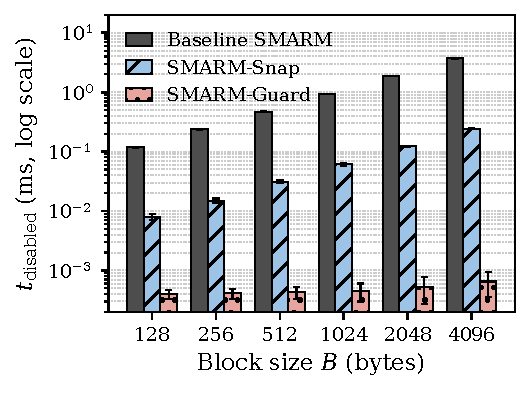
\includegraphics[width=.8\linewidth]{tdisabled_three_log.pdf}
  \caption{Mean non-interruptibility period (\tdis{}) across designs
  on a logarithmic scale. Error bars show standard deviation.}
  \label{fig:tdisabled}
\end{figure}

\begin{table}[t]
  \centering
  \caption{Mean and standard deviation of \tdis{} over ten attestation
  rounds, measured using the DWT cycle counter at $110$~MHz.
  The SMARM baseline and \smarmcopy{} are reported in ms;
  \smarmlock{} is reported in $\mu$s.}
  \label{tab:tdisabled}
  \small
  \setlength{\tabcolsep}{2.8pt}
  \begin{tabularx}{\columnwidth}{@{}lXXXXXX@{}}
    \toprule
    \textbf{$B$ (bytes)}
      & 128 & 256 & 512 & 1024 & 2048 & 4096 \\
    \midrule
    SMARM baseline mean (ms)
      & 0.119 & 0.236 & 0.469 & 0.936 & 1.868 & 3.732 \\
    SMARM baseline std. (ms)
      & 0.0015 & 0.0023 & 0.0031 & 0.0035 & 0.0055 & 0.0085 \\
    \midrule
    \smarmcopy{} mean (ms)
      & 0.008 & 0.015 & 0.031 & 0.061 & 0.122 & 0.243 \\
    \smarmcopy{} std. (ms)
      & 0.0009 & 0.0012 & 0.0017 & 0.0024 & 0.0031 & 0.0038 \\
    \midrule
    \smarmlock{} mean ($\mu$s)
      & 0.40 & 0.41 & 0.43 & 0.45 & 0.52 & 0.65 \\
    \smarmlock{} std. ($\mu$s)
      & 0.07 & 0.08 & 0.10 & 0.15 & 0.25 & 0.29 \\
    \bottomrule
  \end{tabularx}
\end{table}


\subsection{Secure Memory Overhead}

\smarmcopy incurs additional Secure RAM overhead because each block must be copied into a protected buffer before it is measured. This overhead is exactly equal to the block size $B$, since the buffer must be large enough to hold one complete memory block.
In contrast, \smarmlock does not require a copy of the measured block and therefore introduces no additional Secure RAM overhead beyond that already required by the SMARM baseline. 


\subsection{Real-Time Availability}

% We evaluate real-time availability using the Frequency Accuracy Ratio (FAR) metric proposed in~\cite{smarmplus2026}, defined as:
% \begin{align*}
%     \mathrm{FAR} = f_{\mathrm{observed}} / f_{\mathrm{baseline}}
% \end{align*}
% where $f_{\mathrm{observed}}$ is the observed execution frequency of a periodic real-time task while attestation is active, and $f_{\mathrm{baseline}}$ is its execution frequency under the same attestation workload but without interrupt disablement. Thus, $\mathrm{FAR}\approx1.0$ indicates that attestation introduces little interference with the execution frequency of the real-time task, whereas a lower FAR indicates increasing interference.

% As shown in~\cite{smarmplus2026}, under a $1000$~Hz real-time workload, the FAR of the SMARM baseline decreases significantly as $B$ increases, particularly when \tdis becomes longer than the task period. 
% In contrast, both \smarmcopy{} and \smarmlock{} maintain $\mathrm{FAR}\approx1.0$ across all evaluated block sizes, including $B{=}4096$~bytes. These results show that the substantial reductions in \tdis{} achieved by our enhancements translate directly into improved real-time availability, allowing high-frequency real-time tasks to continue executing with negligible interference during attestation.

We evaluate real-time availability using the Frequency Accuracy
Ratio $\mathrm{FAR}=f_{\mathrm{observed}}/f_{\mathrm{baseline}}$
~\cite{smarmplus2026}, where $f_{\mathrm{observed}}$ is the activation
frequency of a periodic FreeRTOS task (\texttt{osDelayUntil},
$1000$~Hz, higher priority than the attestation wrapper) during an
attestation round, and $f_{\mathrm{baseline}}$ is the nominal
$1000$~Hz rate.\oak{this is incorrect. $f_{\mathrm{baseline}}$ should be frequency of this task when no interrupts are disabled. Also you should mention that we use one real-time task with 1000Hz and run SMARM while the task is running. Currently, it doesnt have enough info to understand the results.}

Table~\ref{tab:far} reports mean FAR over ten rounds
using the same evaluation setup with $|M|{=}128$~KiB. The SMARM
baseline maintains $\mathrm{FAR}=1.000$ for $B\leq1024$, where
\tdis{} remains below the $1$~ms task period, but drops to $0.54$
and $0.27$ at $B{=}2048$ and $4096$, respectively, as \tdis{}
exceeds the task period. Both \smarmcopy{} and \smarmlock{} keep
$\mathrm{FAR}=1$ for every tested~$B$, including the highest $B=4096$.

% NEW (M4):
\begin{table}[ht]
  \centering
  \caption{Measured FAR at $1000$~Hz ($|M|{=}128$~KiB, ten rounds).}
  \label{tab:far}
  \small
  \setlength{\tabcolsep}{3.5pt}
  \begin{tabularx}{\columnwidth}{@{}lXXXXXX@{}}
    \toprule
    \textbf{$B$} & 128 & 256 & 512 & 1024 & 2048 & 4096 \\
    \midrule
    Baseline & 1.00 & 1.00 & 1.00 & 1.00 & 0.54 & 0.27 \\
    \smarmcopy & 1.00 & 1.00 & 1.00 & 1.00 & 1.00 & 1.00 \\
    \smarmlock & 1.00 & 1.00 & 1.00 & 1.00 & 1.00 & 1.00 \\
    \bottomrule
  \end{tabularx}
\end{table}

% \begin{table}[t]
%   \centering
%   \caption{Comparison of attestation approaches (TrustZone-M / FreeRTOS).}
%   \label{tab:ra_comparison}
%   \small
%   \renewcommand{\arraystretch}{1.15}
%   \setlength{\tabcolsep}{8pt}

%   \begin{tabular}{@{}lccc@{}}
%     \toprule
%     \textbf{Approach} &
%     \makecell{\textbf{FAR $\approx 1$} \\ \textbf{at 1\,kHz}} &
%     \makecell{\textbf{Extra Secure} \\ \textbf{RAM}} &
%     \makecell{\textbf{\tdis} \\ \textbf{Scale}} \\
%     \midrule
%     Traditional RA~\cite{eldefrawy2012smart,eldefrawy2017hydra,nunes2019vrased} &
%     \texttimes & 0 & $10^{2}$--$10^{3}$\,ms \\

%     SMARM (TZ-M baseline)~\cite{smarmplus2026} &
%     Partial & 0 & $10^{-1}$--$10^{0}$\,ms \\

%     \textbf{\smarmcopy} (ours) &
%     \checkmark & $B$ & $\sim10^{-2}$--$10^{-1}$\,ms \\

%     \textbf{\smarmlock} (ours) &
%     \checkmark & 0 & $\sim\!\mu$s \\
%     \bottomrule
%   \end{tabular}
% \end{table}

\begin{table}[t]
  \centering
  \caption{Comparison of attestation approaches (TrustZone-M / FreeRTOS).}
  \label{tab:ra_comparison}
  \small
  \renewcommand{\arraystretch}{1.15}
  \setlength{\tabcolsep}{2.5pt}

  \begin{tabularx}{\columnwidth}{@{}
    >{\raggedright\arraybackslash}X
    c c c@{}}
    \toprule
    \textbf{Approach} &
    \makecell{\textbf{FAR $\approx 1$} \\ \textbf{at 1\,kHz}} &
    \makecell{\textbf{Extra Secure} \\ \textbf{RAM}} &
    \makecell{\textbf{\tdis} \\ \textbf{Scale}} \\
    \midrule

    Traditional RA~\cite{eldefrawy2012smart,eldefrawy2017hydra,nunes2019vrased} &
    \texttimes & 0 & $10^{2}$--$10^{3}$\,ms \\

    SMARM (TZ-M baseline)~\cite{smarmplus2026} &
    Partial & 0 & $10^{-1}$--$10^{0}$\,ms \\

    \textbf{\smarmcopy} (ours) &
    \checkmark & $B$ & $\sim10^{-2}$--$10^{-1}$\,ms \\

    \textbf{\smarmlock} (ours) &
    \checkmark & 0 & $\sim\!\mu$s \\
    \bottomrule
  \end{tabularx}
\end{table}

\subsection{Total Attestation Runtime}

Reducing \tdis{} does not necessarily reduce total attestation time, as the MAC computation over $|M|$~KiB of memory remains the dominant cost.
As shown in Table~\ref{tab:attest_runtime}, the total attestation times of the SMARM baseline and \smarmlock{} differ by only a few milliseconds across the evaluated values of $B$.
Meanwhile, \smarmcopy{} incurs an additional $7$-$8$~ms due to memory copying.
We consider these differences are relatively small compared to the overall attestation time.



\begin{table}[!ht]
  \centering
    \caption{End-to-end attestation time (ms), $|M|{=}128$~KiB,
    ten rounds, no concurrent real-time task
    (standard deviation $<1$~ms).}
  \label{tab:attest_runtime}
  \small
  \setlength{\tabcolsep}{3.5pt}
  \begin{tabularx}{\columnwidth}{@{}lXXXXXX@{}}
    \toprule
    \textbf{$B$ (bytes)} & 128 & 256 & 512 & 1024 & 2048 & 4096 \\
    \midrule
    SMARM baseline  & 142 & 131 & 125 & 123 & 121 & 120 \\
    \smarmcopy  & 149 & 138 & 132 & 130 & 128 & 128 \\
    \smarmlock & 140 & 130 & 125 & 122 & 121 & 121 \\
    \bottomrule
  \end{tabularx}
\end{table}


\subsection{Results Summary}
\label{sec:guidance}
% \begin{table}[t]
%   \centering
%   \caption{Comparison of attestation approaches.}
%   \label{tab:ra_comparison}
%   \renewcommand{\arraystretch}{1.08}
%   \footnotesize
%   \setlength{\tabcolsep}{2pt}
%   \begin{tabularx}{\columnwidth}{@{}
%       >{\raggedright\arraybackslash}p{0.30\columnwidth}
%       c c c
%       c@{}}
%     \toprule
%     \textbf{Approach} &
%     \makecell{\textbf{RT} \\ \textbf{safe}} &
%     \makecell{\textbf{Extra} \\ \textbf{Secure RAM}} &
%     \makecell{\textbf{\tdis} \\ \textbf{magnitude (ms)}} &
%     \makecell{\textbf{RTOS} \\ \textbf{support}} \\
%     \midrule

%     Traditional RA~\cite{eldefrawy2012smart,eldefrawy2017hydra,nunes2019vrased} &
%     \texttimes &
%     0 &
%     $\sim 10^{3}$ &
%     \texttimes \\

%     SMARM~\cite{carpent2018smarm} &
%     Partial &
%     0 &
%     $\sim10^{-1}$--$10^{0}$ &
%     \texttimes \\

%     \textbf{\smarmcopy} &
%     \checkmark &
%     $B$ &
%     $\sim10^{-2}$--$10^{-1}$ &
%     \checkmark \\

%     \textbf{\smarmlock} &
%     \checkmark &
%     0 &
%     $\sim 10^{-3}$ &
%     \checkmark \\

%     \bottomrule
%   \end{tabularx}
% \end{table}

% Table~\ref{tab:ra_comparison} summarizes our two enhancements and compares them with traditional RA and the SMARM baseline. Both \smarmcopy{} and \smarmlock{} substantially reduce \tdis{}, making them well suited to real-time applications with RTOS support. In particular, \smarmlock{} reduces \tdis{} to the microsecond range, making the attestation process nearly fully interruptible.

% These improvements, however, come with different trade-offs. \smarmcopy{} requires an additional Secure buffer of size $B$ to store the snapshot. In contrast, \smarmlock{} requires no additional Secure RAM, but ephemerally makes the block under measurement inaccessible to Non-Secure software. Consequently, a concurrent Non-Secure task that attempts to access this block during its measurement may experience a fault, which could indirectly affect its real-time execution. This represents a trade-off between Secure-memory overhead and potential memory-access interference. In practice, \smarmlock{} is therefore most suitable when the attested region can tolerate such faults, whereas \smarmcopy{} provides a preferable alternative when uninterrupted Non-Secure access to the attested memory is required.


\ben{Table~\ref{tab:ra_comparison} summarizes the trade-off: \smarmcopy{} needs a Secure buffer of size~$B$, while \smarmlock{} needs none and is evaluated on a dedicated Non-Secure attested region; if continuous Non-Secure access is required during measurement, \smarmcopy{} or the SMARM baseline is preferable.}\oak{we should also mention \tdis -- remember the title of this paper. \tdis should be the main show here.}

\section{Related Work}
\label{sec:related}

Traditional RA techniques~\cite{eldefrawy2012smart,nunes2019vrased,eldefrawy2017hydra} commonly disable interrupts throughout the entire memory measurement to preserve temporal consistency and prevent malware from modifying or relocating itself during attestation. However, the resulting long non-interruptibility period can interfere with time-sensitive operations.

SMARM~\cite{carpent2018smarm}, PRoM~\cite{aman2021prom}, and HAtt~\cite{aman2018hatt} relax this requirement through \emph{shuffled measurement}, allowing interrupts between consecutive block measurements. Nevertheless, each individual block measurement must still execute atomically, leaving the non-interruptibility period whose duration depends on the block-measurement time.
Our work is complementary to these approaches and specifically targets this remaining per-block non-interruptibility.

Other work addresses interruptibility via runtime attestation, trusted monitoring, or dedicated hardware support~\cite{isc-flat,asap,ida2024,lo-fat,litehax,atrium}.
In contrast, our work reduces the remaining non-interruptibility of \emph{shuffled memory measurement} on commodity TrustZone-M hardware without requiring custom hardware support.




% ================================================================
% \section{Conclusion}
% \label{sec:conclusion}
% % SMARM improves remote attestation for real-time systems by allowing interrupts between memory blocks, but hashing each block with interrupts disabled can still stall time-critical work when blocks are large.
% % We proposed two enhancements on FreeRTOS with TrustZone-M: \smarmcopy{} snapshots each block into Secure memory and hashes it with interrupts enabled, while \smarmlock{} briefly guards each block via SAU updates and hashes in place.
% % Our results reduce the per-block non-interruptibility period by about one order of magnitude with \smarmcopy{} and two to three orders with \smarmlock, moving toward fully interruptible shuffled measurement.

\section{Conclusion}
\label{sec:conclusion}
% SMARM improves remote attestation for real-time systems by allowing
% interrupts between memory blocks, but hashing each block with interrupts
% disabled can still stall time-critical work when blocks are large.
% We propose two complementary enhancements on FreeRTOS with TrustZone-M.
% \smarmcopy{} shortens the non-interruptibility period to a brief Secure
% memory copy, then hashes with interrupts enabled; it needs a Secure buffer
% the size of one block and adds roughly thirty milliseconds to a full
% attestation round.
% \smarmlock{} shortens that period further without the additional storage requirement by briefly
% making each block unavailable to Non-Secure software through SAU updates,
% then hashing the block in place with interrupts enabled.
% Our experimental results show reductions of the non-interruptibility period around one order of magnitude with \smarmcopy and two to three orders with \smarmlock, representing progress toward fully interruptible shuffled measurement for remote attestation.

SMARM allows interrupts between memory blocks, but per-block hashing can still stall high-frequency real-time tasks when blocks are large. We propose two complementary FreeRTOS/TrustZone-M enhancements. \smarmcopy{} shortens the non-interruptibility period to a brief Secure memory copy at the cost of a Secure buffer of size~$B$. \smarmlock{} instead uses brief SAU reconfigurations with no extra buffer, assuming that the attested region cannot be modified during measurement. On our platform, \smarmcopy{} reduces \tdis{} by about one order of magnitude ($\sim\!\!15\times$) and \smarmlock{} by roughly three to four orders at large~$B$; both keep measured FAR~$=1.0$ at $1000$~Hz in our evaluation.


\section*{Acknowledgments}
This work was supported by the College of Computing,
Prince of Songkla University, Phuket Campus.


% SMARM improves RA interactivity by allowing interrupts between blocks,
% but its per-block interrupt-disabled hash still yields a long
% \tdis{} for large~$B$ on FreeRTOS/TrustZone-M.
% \smarmcopy{} shortens that window to a Secure memory copy
% and restores FAR~$\approx 1.0$ under a $1000$~Hz workload, at the cost
% of a Secure buffer of size~$B$.
% \smarmlock{} achieves a still shorter \tdis{} without that buffer by
% making each measured block ephemerally unavailable to Non-Secure
% software via brief SAU updates, then hashing in place with interrupts
% enabled; it likewise maintains FAR~$\approx 1.0$ at $1000$~Hz across
% the evaluated block sizes.
% Both enhancements preserve SMARM's security properties~(S1)--(S3):
% controlled Secure/NSC entry with integrity of each block capture,
% secrecy of~$k$, and privacy of the measurement order~$\sigma$.
% In practice, prefer \smarmcopy{} when Secure RAM of size~$B$ is
% available or the SAU must remain fixed after boot, and prefer
% \smarmlock{} when a dedicated Non-Secure attested region~$|M|$ can absorb
% brief SAU attribution changes without an extra Secure buffer.

{\footnotesize
\bibliographystyle{IEEEtran}
\bibliography{citation}
}

\end{document}
